% !TEX root = DesignDocument.tex

\chapter{User Stories,  Requirements, and Product Backlog}



\section{Overview}


The purpose of this document is to give the reader a thorough understanding of
not only the product created by this senior design team, but also of the
process behind developing the project. This spans project purpose, user
requirements, team organization, design, implementation, testing, project
management, and user documentation.

While creating this document, we have endeavored to make it detailed enough
that it could be the sole resource needed by a similar team to create an exact
replica of our product.

The purpose of this product is to heighten the education experience for
students, expecially in scenarios that require 3D visualization. The goal is to
make 3D content delivery simple so that instructors can take advantage of the
technology and give their students a more immersive, engaging experience.

Once we had our purpose for the product set out, it was a matter of getting
ourselves organized and creating clear definitions of what needed to be done.
In order to define actionable items for our product backlog, we had to define
the requirements for our project. This in turn was defined through user stories.

% The user stories are provided by the stakeholders. You will create the
% backlogs and the requirements, and document here. This chapter should
% contain details about each of the requirements and how the requirements are 
% or will be satisfied in the design and implementation of the system.

% Below: list, describe, and define the requirements in this chapter.  There
% could be any number of sub-sections to help provide the necessary level of
% detail.


\section{User Stories}

User stories are collected through conversations with the stakeholders and
regularly displaying what the team has accomplished. The senior design team had
weekly meetings with the client to review progress on the project. The team met
with other faculty related to the project as necessary in order to receive
feedback.

The starting point for the requirements and user stories for this project came
from the a grant proposal by Dr. McGough and other SD Mines faculty,
which can be found in ~\autoref{ch:support}. Over the course of several
meetings and conversations with the professors on the grant, the
requirements for our product were defined.

An example user story from the grant is as follows: "As a Calc III
professor, I would like to provide visualizations of 3D objects so that
students can find the volume of an object by being able to view the object
from different angles, and being able to slice the object's volume."

Some base requirements identified for the platform include:
\begin{itemize}
	\item A website to manage files
	\item Support for 3D files exported from CAD programs commonly used in STEM
	\item Automatic file conversion
	\item Render files on the Microsoft HoloLens
	\item Render files on an Android mobile device
\end{itemize}

At the advice of faculty advisors, the user stories were grouped into three 
development rounds. User story defines a test as appropriate. More detail on tests can be found in Chapter \ref{ch:testing}.

\subsection{Phase 1: Senior Design I}

User Stories:
\begin{itemize}
	\item As an SD Mines faculty member, I want to:
		\begin{itemize}
			\item Upload a 3D file to the cloud.
			\item Retrieve the file in the proper format.
			\item Download a QR code for a model.
			\item Log in to a secure account and view my uploaded files.
			\item Choose files to be private or public.
			\item Browse and download public files.
		\end{itemize}
\end{itemize}
Tests:
\begin{itemize}
	\item Conversion of multiple types of 3D models.
	\item Viewing and manipulating the models on the HoloLens.
	\item Generation of a unique QR code associated with each model.
	\item Upload and download process for a 3D model.
\end{itemize}

\subsection{Phase 1: Senior Design II}

User Stories:
\begin{itemize}
	\item As a user, I want to:
	\begin{itemize}
		\item View surface materials on 3D model.
		\item Use an Android phone for scanning QR codes and viewing models.
		\item Switch between models quickly in the AR device.
	\end{itemize}
\end{itemize}
Tests:
\begin{itemize}
	\item Upload a file and verify that the AR tag received links to the correct
	model.
	\item Test privacy rules and visibility for files by creating multiple 
	profiles with different privacy settings.
	\item Gather 3D models of multiple file types and test the rendering of 
	textures and surface materials.
	\item Verify that privacy settings work and users are able to download files
	according to permissions on those files.
\end{itemize}


\section{Requirements and Design Constraints}

% we could include an intro here

\subsection{System Requirements}

% What are they? How will they impact the potential design? Are there alternatives
The basic system requirements to use the website are to have a web browser 
installed with internet access.  The user must have access to modeling software 
or a method to create/provide 3D models to the website.

In order to fully use the product, a user must have an Augmented Reality device.
Each device may have different system requirements. Some AR devices such as the 
HoloLens or AR compatible smartphones will not require a computer to run off. 
However, some AR devices require to be tethered to a computer. Usually, 
manufacturers detail a set of quite high minimum specifications for a computer 
that can be used

The Meta 2 is an example of a headset that requires a seperate computer in order
to run.  In our research we found that the Meta 2 specified one of the highest 
recommended specifications among popular VR headsets. This makes it a good 
example for system specifications that would run an AR application smoothly. 
The minimum and recommended specifications are listed below. The list was crated
in November 2017, and can be found in table 
\ref{table:metatwosystemrequirements}.

\begin{table}[H]
	\centering
	\begin{tabular}{ | c | c | c | }
		\hline
		& Minimum & Recommended \\ \hline
		OS & Windows 10 (64 bit) & 	Windows 10 (64 bit) \\ \hline
		CPU & Intel i7-4770 & Intel i7-6700 \\ \hline
		RAM & 8GB DDR3 & 16GB DDR4 \\ \hline
		GPU & NVIDIA GTX 960 & NVIDIA GTX 970 \\ \hline
		Hard Drive & 2GB Free Space & 2GB+ Free Space \\ \hline
		I/O Ports & 1X HDMI 1.4b and 2X USB 3.0 ports & 1X HDMI 1.4b and 2X USB 3.0 ports \\ \hline
		3D Engine & Unity 5.6 or higher & Unity 5.6 or higher \\ \hline
	\end{tabular}

	\caption{Meta 2 System Requirements}
	\label{table:metatwosystemrequirements}
\end{table}

More up to date requirements can be found on the Meta 2 website at: 
\url{https://buy.metavision.com/}

\subsection{Network Requirements}

Being able to take advantage of the features in this product will need a network
that is able to easily upload and download 3D models. The user will need to have
both their computer and AR viewer configured for network access.

\subsection{Development Environment Requirements}
% What are they? Is the system supposed to be cross-platform?
\begin{itemize}
	\item Windows 10 - To be able to develop for the HoloLens.
	\item Visual Studio 2017 Enterprise with ASP.NET MVS, Azure and Unity tools.
	\item Unity Personal
	\item HoloToolkit - Unity Set of tools for Hololens development with Unity.
	\item Assimp library
	\item FBX SDK
\end{itemize}


\subsection{Project Management Methodology}
% The stakeholders might restrict how the project implementation will be managed.
%  There may be constraints on when design meetings will take place. There might
% be restrictions on how often progress reports need to be provided and to whom.
The team has a weekly meeting with our client representative Jared Johnson and 
our faculty advisors, Dr. McGough and Dr. Karlsson. At these meetings we provide
progress reports and discuss any design modifications and blocks.

The team for this project has self-organized and decided on Brady Shimp as a
Scrum Master and Cheldon Coughlen as Team Lead. We use GitHub for the majority 
of our project management tools, issue tracking being the main feature.

% \section{Specifications}


% Any specifications that need to be understood? Put it here.


\section{Product Backlog}


This is the entire backlog for the project, including each actionable item we 
have completed or will be working on. New items and checkpoints will be added 
here as they come up.

\begin{itemize}
\item Take in files from Maple and convert them to stored file type.
\item Create website to upload and download 3D models
\item \textbf{Checkpoint One:} Create wireframes, documentation for presentation 1.
\item Host conversion software on the website.
\item Test viewing 3D objects on the HoloLens.
\item Manually create unique QR codes for each file. 
\item \textbf{Checkpoint Two:} Create wireframes, demos, documentation for presentation 
2.
\item Automatic QR code generation.
\item Detect QR code and download file.
\item Create and manage user profiles.
\item Allow users to control visibility of uploaded models.
\item HoloLens application development to view downloaded 3D model and interact 
with it.
\item \textbf{Final Checkpoint:} Prepare materials for design fair.
\end{itemize}

\subsection{Backlog Tracker}

We manage our backlog using GitHub's project board. Using GitHub's system is 
convenient as we also use it to host our code repository. Items from our backlog 
are added to the backlog column of the project board. They are sometimes broken 
up into smaller issues if the feature is large and can be worked on by multiple 
developers.

When the issue is ready to be worked on, it is taken from the backlog and 
assigned to a developer. The project board has three other sections: 
'Work in Progress', 'QA', and 'Ready' as seen in Figure 
~\ref{fig:ProjectTaskBoard}. Once the developer begins working on it, 
they move it to 'Work in Progress'. When they have the issue taken care of, they
move it to 'QA' and assign it to a developer that has not worked on the issue, 
but has the background to test it. Once it is verified that the issue has been 
fixed, it is moved to 'Ready'. If any problems arise while testing the solution,
it is communicated to the developers who worked on it and the issue is moved 
back to 'QA'.

\begin{figure}[H]
    \centering
    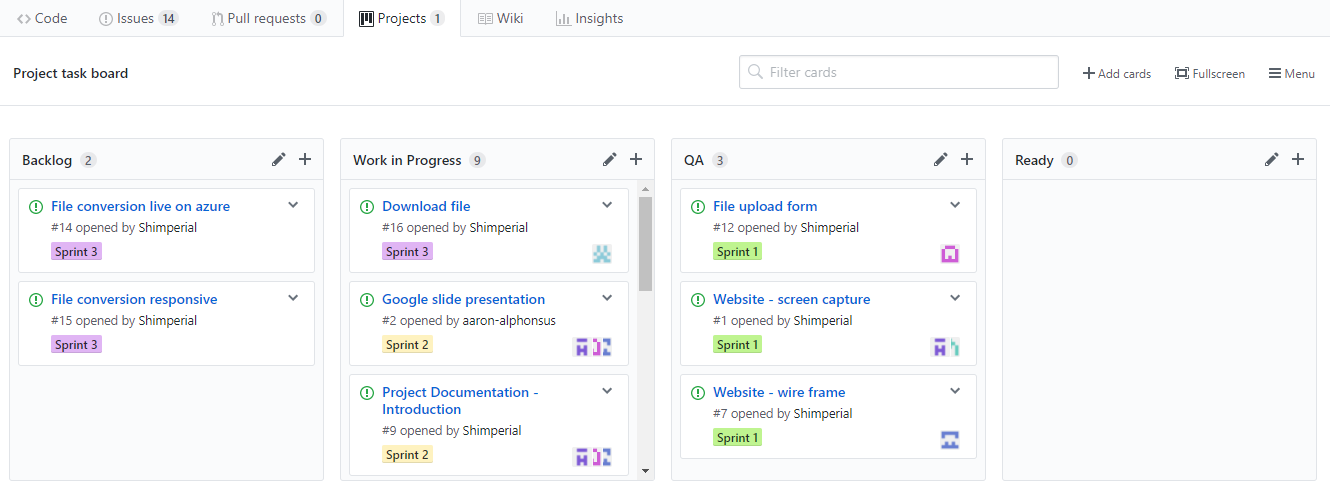
\includegraphics[width=\textwidth]{ProjectTaskBoard.png}
    \caption{Project Task Board}
    \label{fig:ProjectTaskBoard}
\end{figure}

By default, just the development team has access to the Sprint and Product 
Backlog on GitHub, but through stand-alone documentation, presentations, and 
other communication, we share this information with our other stakeholders. 
We can provide access to the actual backlog we maintain on the GitHub repository
on request.

\subsection{Sprints}
The project is encompassed by 13 Sprints - 6 in the Fall semester and 7 in the 
Spring semester. Each sprint is defined to be two weeks long. 
For each sprint, we define a backlog and assign developers to tasks. We also 
define deliverables that will be prepared by the end of the sprint. At the end 
of each sprint, we reflect on the successes and failures, and look forward to 
what needs to happen in subsequent sprints.


\section{Research or Proof of Concept Results}


To some extent, the work done in our first semester is centered on giving our 
stakeholders a proof of concept so that they can begin to drive the requirements
of the project in the future. We had a couple of meetings with faculty to demo 
what we were able to create in VR and AR so that they could see the capabilities
of the technology, and think about how they could integrate it in their 
classroom. At the end of our first semester of development, we will have an MVP
to demonstrate the proof of concept. Our presentations through the semester have 
contained wireframes and demos that reflect the features our MVP will have.

With regards to research and system design, the team has been doing both
concurrently. This is possible since Dr. McGough provided the team with a 
high-level view of the entire system and the data flow before we began the 
project. This meant that the team able to focus on researching and implementing 
smaller pieces of the system. 


\section{Supporting Material}


As mentioned earlier, the original mobile computing grant proposed by Dr. 
McGough and other SD Mines faculty is the main source that has driven the
specifications of the product. We have provided the grant in 
~\autoref{ch:support} so that the reader has a good understanding of the
motivation behind this product, and what the long-term goals are.

